For each constraint, not transformed into a oneway constraint, auxiliary variables are introduced as invariants and an 
invariant for violation degree is created. The are created by calling the method \method{createInvariants} of each 
constraint and the algorithm for \class{Linear} was shown in subsection \ref{sub_cons}. \\
The dependency directed graph (\emph{DDG}) $G=(V,A)$ is made of a set of vertices $V$ representing all independent 
variables and all invariants. To ease the notation we say the value of vertex $v \in V$ is the value of the variable or 
invariant it represents. \\
The vertex $v \in V$ has an outgoing arc $vu \in A$ to vertex $u \in V$ if and only if the value of $u$ is directly 
dependent on the value of $v$. The vertices representing independent variables never have an ingoing arc. \\ 
The graph can be illustrated with all the variable vertices to the left with outgoing arcs going right to vertices 
representing invariants. \\  
If a variable is defined by a oneway constraint the variable vertex is removed from $G$ since the value of that 
variable is given by the invariant representing it. \\  
%From now on when talking about vertices in $G$ it refers to the variable, invariant or constraint it represents unless 
%other stated. \\
%The variables are non-fixed and non-defined and only have outgoing arcs. 
%Variables and invariants has an outgoing arc to the invariants that 
%depends on their value. \\ 
The DDG is used when doing local search and contains dependencies of variables and invariants. The 
graph $G$ is also used to build 
the propagation queues described in subsection \ref{sec_propaqueue}. The idea of a graph representing the relationship 
between invariants comes from Comet \cite[p. 97]{comet} and OscaR\cite[p. 7-9]{oscar}. \\
To illustrate how the DDG is made an example of a model with three variables and a two constraint will 
illustrate it. \\ 
\begin{center}
\begin{tabular}{rlr}
$ c_1: $&$x_1 + x_2 - x_3 $&$= 1$ \\
$ c_2: $&$2x_2 + x_3 $&$\leq 2$ \\
\end{tabular} 
\end{center}
The variable $x_3$ can be defined as an invariant $y_1$ by transforming $c_1$ to a oneway constraint $c_1': x_3 = 
x_1+x_2-1$. Once variable $x_3$ is defined by a oneway constraint $x_3$ are removed from the graph and replaced by 
invariant $y_1$. The variables $x_1$ and $x_2$ defines $y_1$ hence they have outgoing arcs to $y_1$. This is 
illustrated in figure \ref{fig_smallG} 
\begin{figure}[t]
\begin{center}
    \begin{tikzpicture}[scale=1]
        \vertex[label=$x_1$](x1) at (0,2) {};
        \vertex[label=$x_2$](x2) at (0,0) {};
        \vertex[label=$y_1$](i1) at (2,1) {};
%         \vertex[label=$c_2$](c2) at (4,0) {};

    \tikzset{EdgeStyle/.style={->}}
        \Edge(x1)(i1)
        \Edge(x2)(i1)
%         \Edge(x2)(c2)
%         \Edge(i1)(c2)
        %\Edge(y1)(c3)
        %\Edge(y2)(c3)
    \end{tikzpicture}
        \captionof{figure}{Small example of DDG}
    \label{fig_smallG}
\end{center}
\end{figure} \noindent
Auxiliary variable can be useful to update constraint violations and in this example we could create an auxiliary 
variable where value is the sum of the left hand side of $c_2$. The auxiliary variable will be represented 
by a \class{Sum} invariant $y_2$ which will be added to $G$. The invariant $y_1$, representing $x_3$, and variable 
$x_2$ have an outgoing arc to $y_2$. A \class{LEQViolation} invariant $y_3$ representing the violation of constraint 
$c_2$ is added as well.
\begin{figure}[b]
\begin{center}
    \begin{tikzpicture}[scale=1]
        \vertex[label=$x_1$](x1) at (0,2) {};
        \vertex[label=$x_2$](x2) at (0,0) {};
        \vertex[label=$y_1$](i1) at (2,1) {};
        \vertex[label=$y_2$](i2) at (4,0) {};
        \vertex[label=$y_3$](i3) at (6,0) {};

    \tikzset{EdgeStyle/.style={->}}
        \Edge(x1)(i1)
        \Edge(x2)(i1)
        \Edge(x2)(i2)
        \Edge(i1)(i2)
        \Edge(i2)(i3)
    \end{tikzpicture} 
    \captionof{figure}{Small example of DDG continued}
    \label{fig_smallG2}
\end{center}
\end{figure}
When changing the value of $x_2$ both invariants need to be updated since they are dependent on the value of $x_2$. 
Invariant $y_2$ is dependent on the value of $y_1$ therefore to avoid updating $y_2$ twice, it is beneficial to 
update $y_1$ before updating $y_2$. This is the ordering given the propagation queue that is discussed in the next 
subsection. \medskip \\
%\end{minipage}
%\boste{start on algorithms}
%The DDG $G$ is initially a bipartite graph where all the decision variables $X$ are vertices in one set and all the 
%constraints $C$ are vertices in the other set. If constraint $c$ applies to a variable $x$ then there is an arc from 
%the vertex representing $x$ to the vertex representing $c$. \\   
In order to avoid circular definitions of invariants dependency directed graph $G$ is made acyclic. A circular 
definition could be if $x_i$ is used to define $x_j$ and vise versa. Then a change in value of $x_i$ would lead to a 
change in value of $x_j$ that again changes the value of $x_i$ and so on.  \\ 
In order to remove circular definitions, all strongly connected components of size two or more in $G$ is found. A 
\emph{strongly connected component} (SCC) is a maximal set of vertices $V^{SCC}$ such that for each pair of vertices 
$(u,v) \in V^{SCC}$ there exist both a path from $u$ to $v$ and a path from $v$ to $u$ \cite[p. 1170]{cormen}. 
Each of these strongly connected components must be broken in order to keep $G$ acyclic, since a SCC consist of at 
least one cycle. A SCC can be broken by removing arcs and/or removing vertices. The arcs $A$ represent relations 
between variables, invariants and constraints and should not be changed. The set of vertices $V^{SCC}$, in a SCC, can 
only be vertices representing invariant since variable only have outgoing arcs and constraint only have ingoing arcs. 
Undefining one of those invariants corresponds to removing one of the vertices, hence breaking the SCC. An invariant can 
be undefined by reintroducing the variable it represents and removing the invariant from the model. The oneway 
constraint used to define the invariant is transformed back into a functional constraint again and is reintroduced in 
the model. \\
For each SCC one of the vertices is chosen and the invariant it represents is undefined. The invariant is chosen in the 
order of lowest domain then highest arity of oneway constraint defining it. If there is ties they are broken at random.
\\  
To find all SCC of size two or more Tarjan's algorithm for finding strongly connected components is used. \boste{cite 
SIAM J. Comput., 1(2), 146–160.}. Tarjan's algorithm has a recursive depth first search behavior when exploring 
vertices and uses a stack when exploring. The stack consist of vertices that has been visited before but not part of a 
strongly connected component yet. The use two counters, first one $index$ is unique in the order they are visited the 
other is $lowlink$ initially the same as $index$. If we go from vertex $v$ to vertex $u$ and $u$ has been visited 
before, $v.lowlink = min(v.index,u.lowlink$. If $u$ has not been visited the search continues from $u$. When all 
neighbors of a vertex $v$ has been explored if $v.index$ is equal to its $v.lowlink$ the stack is popped until $v$ is 
popped. All the vertices $V^{SCC}$ popped from the stack is a strongly connected component. \\
The algorithm has been modified to give each variable a time stamp when they are popped from the stack as well. That 
time stamp gives an ordering of the invariants used to create the propagation queues described in the next subsection. 
The time stamp is updated each time the algorithm is restarted. \\
Removing the fewest possible invariants such that there are no cycles in $G$ corresponds to solving the minimum 
feedback arc set problem and is known to be NP-hard \cite[p.9]{oscar}. In order to reduce the construction time a 
greedy approach is chosen. \\
Once these strongly connected components are broken there is still no guarantee that $G$ is a directed acyclic graph 
(DAG). A strongly connected component can be made of several cycles and it might not be sufficient just to break all 
SCC found by Tarjans algorithm initially. The process of finding SCC with Tarjans algorithm and then 
breaking these strongly connected components is repeated until no strongly connected components (of size two or more) 
is found by Tarjans algorithm. \medskip \\  
The only vertices that can make strongly connected components are the vertices representing invariants, more 
specifically only the invariants that define a variable. Therefore the check for strongly connected components are done 
before other invariants are added. After they are added Tarjans algorithm is repeated to give all invariants a 
time stamp. \\ 
The first tiebreaker in algorithm \ref{algo_makeoneway} is used as a heuristic to reduce the number of cycles 
generated.  \\





%A circular definition could be if $x_i$ is used define $x_j$ and conversely \boste{vise versa?} then a change in value 
%of $x_i$ would lead to a change in value of $x_j$ that again changes the value of $x_i$ and so on. \\
%Cycles are found with . For each of the 
%strongly connected components of size two or more one of the vertices should be removed. Removing a vertex corresponds 
%to undefine an invariant and reintroduce the transformed constraint. After removing one vertex for each scc Tarjans 
%algorithm is used to find new scc if any. This is repeated until no scc of size two or more is found. Tarjans 
%algorithm 
%is modified a bit to give each vertex a time stamp when it becomes a part of a scc hence the last time it is visited. 
%This time stamp can be used for a topological sorting of the vertices once $G$ is a directed acyclic graph 
%(\emph{DAG}). 
%It gets complicated to compute the propagation queues if there exist a strongly connected component in $G$. 
%Only invariant vertices can be part of a strongly connected component of size at least two, since variables vertices 
%only have outgoing arcs and constraint vertices only have ingoing arcs. This indicates that there could be circular 
%definition of variables. Because of this we want to avoid ending up with strongly connected components in the graph 
%$G$. \medskip \\
%This is not the most efficient way of finding cycles, an algorithm with better complexity is described by \boste{cite 
%SIAM J. Comput., 4(1), 77–84, Tarjan has complexity O(|V|+|A|) not sure it is actually better to find elementary 
%cycles. Talk about finding minimum number of vertices to remove. Minimum feedback, NP-hard}. \\ 


%Consider the following three constraints as a small example. \boste{Should the example be introduced before the 
%algorithms?}
%\begin{center}
%\begin{tabular}{rlr}
%$ c_1: $&$2x_1 + y_2 -y_1 $&$= 2$ \\
%$ c_2: $&$2x_1 - y_2 $&$= 2 $ \\ 
%$ c_3: $&$x_1 +y_1 +y_2 $&$\leq 5 $
%\end{tabular} 
%\end{center}
%At first $y_1$ cannot be defined by a \oneway but $y_2$ can be defined by $c_2$ and then $y_1$ can be defined by 
%$c_1$. 
%The order in which the \oneway are created matters. \boste{Not finished here, continue tomorrow morning} 
%\begin{center}
%    \begin{tikzpicture}[scale=1]
%        \vertex[label=$x_1$](x1) at (-1,1) {};
%        \vertex[label=$y_1$](y1) at (3,2) {};
%        \vertex[label=$y_2$](y2) at (1,0) {};
%        %\vertex[label=$c_3$](c3) at (5,1) {};
%         %\vertex[label=$c_2$](c2) at (5,0) {};
%    \tikzset{EdgeStyle/.style={->}}
%        \Edge(x1)(y1)
%        \Edge(y2)(y1)
%        \Edge(x1)(y2)
%        %\Edge(x1)(c3)
%        %\Edge(y1)(c3)
%        %\Edge(y2)(c3)
%    \end{tikzpicture}
%\end{center}

%algorithm \ref{algo_defintvar} first check if $y_1$ can be defined by a \oneway which it cannot since $c_1$ applies to 
%two integer variables. Then $y_2$ cannot be defined by $c_1$ but can be defined by $c_2$. Then $c_2$ is transformed 
%into a \oneway $c_2'$ that defines $y_2$ and it is added to the DDG $G$, $c_2: y_2 = 2x_2 -2$. T  


% \floatname{algorithm}{Finding One-way constraints}
%\begin{algorithm}[ht]
% \caption{O$(|V|^2C_{mav}$O$($\method{canBeMadeOneway()}$)$}
% \begin{algorithmic}\label{updateGraph1}
%  \STATE{$Q = \emptyset$}
%  \STATE{$V = $ model.getVariables()}
%  \STATE{V.sort()}
%  \STATE{\bool change = \true }
%  \WHILE{change}
%    \FOR{\var var in $V$}
%      \FOR{\cons cons in var.usedInConstriant()}
%	\IF{\method{canBeMadeOneway(var, cons)}}
%	  \STATE{V.remove(var)}
%	  \STATE{$Q.psuhback($var$)$}
%	  \STATE{\Break }
%	\ELSE
%	\STATE{change = \\false}
%	\ENDIF
%      \ENDFOR
%    \ENDFOR
%   % \STATE{laxer$++$}
%%{$j\leftarrow 1$ \TO $i-1$}
%  \ENDWHILE
% \end{algorithmic}
%
%\end{algorithm}


% \floatname{algorithm}{}
%\begin{algorithm}[ht]
% \caption{\bool \method{canBeMadeOneway}(\var \text{var}, \cons cons) \qquad O$(V_{mav} + $O$($\method{makeOneway}$))$}
% \begin{algorithmic}\label{updateGraph1}
% \IF{cons.isOneway()}
%  \RETURN \\false
%  \ENDIF
% \STATE{\Int notDefined = 0} 
% \FOR { \var v in cons.getVariables}
% \IF{v.isInteger()}
%  \IF{!v.isDefinedBxOneway}
%  \STATE{notDefined++}
%  \ENDIF
%  \ENDIF
%  \IF{notDefined $> 1$}
%    \RETURN \\false  
% \ENDIF
% \ENDFOR
% \STATE{\Int coef = var.getCoefficient(cons)}
% \STATE{\Int objCoef = var.getObjectiveCoefficient()}
% 
% \IF{cons.Relation = EQ \OR coef$\cdot$objCoef $< 0$}
%    \STATE{\method{makeOneway}(\var var, \cons cons)}
%    \RETURN \true
% \ENDIF
% \RETURN \\false
% \end{algorithmic}
%\end{algorithm}


% \floatname{algorithm}{}
%\begin{algorithm}[ht]
% \caption{\method{makeOneway}(\var \text{var}, \cons cons) \qquad O$(V_{mav})$}
% \begin{algorithmic}\label{updateGraph1}
% \STATE{variables = cons.getVariables()-var}
% \STATE{coefficients = cons.getCoefficient-var.coefficients}
% \STATE{\Int coef = var.getCoefficient(cons)}
% \IF{coef $\neq$ -1}
% \STATE{coefficients = $\frac{-1}{coef}\cdot$ coefficients}
% \ENDIF
% \STATE{\invar invar$(variables, coefficients)$}
% \FOR{\var v in variables}
%  \IF{v.isDefinedBxOneway}
%    \STATE{\invar inv = v.oneway}
%    \STATE{inv.updateList.pushback(invar)}
%  \ELSE
%  \STATE{v.updateList.pushback(invar)}
%  \ENDIF
%   \ENDFOR
%   \STATE{cons.isOneway = \true }
%   \STATE{cons.defines = invar }
%   \STATE{var.setDefinedBx(invar,cons)}
%   \STATE{model.add(invar)}
%   \STATE{invar.currentvalue = -cons.getArgument(1)} 
% \end{algorithmic}
%\end{algorithm}
  

%First all integer variables $Y$ in the CSOP $\mathbb{P}$ \boste{Should I call the models CSOP or just model?} get 
%defined by oneway constraints by algorithm \ref{algo_makeints}. If some of the integer variables cannot be defined 
%\boste{Currently report fail and exit}. 
%\\ 
%\IncMargin{1em}
%\begin{algorithm}[H]
%\SetKwData{Oneway}{oneway}
%\SetKwFunction{makeIntVarOneway}{makeIntVarOneway}
%\SetKwFunction{Next}{next}\SetKwFunction{Constraints}{Constraints}\SetKwFunction{Remove}{remove}
%\SetKwFunction{intVarCanBeMadeOneway}{intVarCanBeMadeOneway}
%\algdata 
%\Input{A set $Y$ of integer variables sorted by decreasing domain size}
%\Output{A CBLS model for local search}
%\BlankLine

%\Bool $change = $ \true\;
%\While{$Y \neq \emptyset$ \textbf{and} $change$}{
%  $change = $\false \;
%  \ForEach{$y_i \in Y$}{
%    \upshape select \Var $y_i$ \upshape from $Y$\;
%    \ForEach{\Con $c_j$ \upshape in $C(y_i)$}{
%      \If{\intVarCanBeMadeOneway{$y_i$,$c_j$}}{
%	\makeIntVarOneway{$y_i$,$c_j$}\;
%	Remove $y_i$ from $Y$\;
%	isOneway($c_j$) = \true \;
%	$change = \true$\;
%	\bre\;
%      }
%    }
%  } \label{false}
%}
%\caption{Defining integer variables by one-way constraints}\label{algo_makeints}
%\end{algorithm}\DecMargin{1em}
%\noindent
%For each of the variables $y_i$ each of the constraints $c_j$ that applies to $y_i$ is checked if it can be made 
%oneway 
%to define $y_i$ until one is found or none can be found. This is done until there are no integer variables left or the 
%remaining integer variables cannot be defined, when the boolean change is false after line \ref{false}. Algorithm 
%\ref{algo_checkintoneway} checks if constraint $c_j$ can be made oneway to define $y_i$ and algorithm 
%\ref{algo_makeintoneway} transforms $c_j$ into a oneway constraint defining $y_i$ and updates the DDG $G$. \\
%Let $\mathcal{F} = \{f_1,f_2,\dots ,f_k\}$ be the family of objective functions. \\
%\IncMargin{1em}
%\begin{algorithm}[H]

%\SetKwFunction{relation}{relation}\SetKwFunction{coeff}{coefficient}
%\SetKwFunction{objcoeff}{objectiveCoefficients}
%\algdata
%\Input{\Var $y_i$ and \Con $c_j$}
%\Output{Boolean}
%\BlankLine
%\If{$c_j$ \upshape already defines a oneway constraint}{\Return{} \false\; \boste{This constraint could be removed in 
%$O(\alpha(c_j))$}}

%int $undefinedIntVar = 0$ \;
%\ForEach{\Var $x$ \upshape in $c_j$}{
%  \If{x is undefined integer variable}{
%    $undefinedIntVar++$\;
%  }
%}
%\If{$undefinedIntVar > 1$ \label{undefined}}{\Return{} \false  \boste{Insures no cycle is created} \; 
%\tcp {else only $y_i$ is undefined integer variable}} 
%\If{$c_j$ \upshape is linear equality}{\Return{} \true}
%\If{\upshape coefficient $c_{ij} \geq 0 $ \label{positivecoef}}{ 
%  \Return{} \false \; 
%}
%\ForEach{ $f_j$  in $\mathcal{F}$ }{
% \If{$f_ij < 0$ \label{objectivecoef}}{
%    \Return{} \false \;
%    \boste{Not sure of to define coefficients in objective functions. coefficient of variable i in constraint j could 
%be $c_{ij}$ but $c_j$ is used for constraint and then all variable $y_i$ should be $y_i$}
%  }
%}
%\Return{} \true\;
% \caption{intVarCanBeMadeOneway( \textsf{Variable} $y_i$, \textsf{Constraint} $c_j$)} \label{algo_checkintoneway}
% \caption{Test if a constraint $c$ can define a variable $x$ } \label{algo_checkoneway}
%\end{algorithm}
%\DecMargin{1em}
%If constraint $c_j$ already defines another variable it cannot be used to define $y_i$. Line \ref{undefined} makes 
%sure 
%that integer variable $y_i$ is not defining another integer variable $y_k$. This limits the model and increases the 
%complexity of algorithm \ref{algo_makeints} because of the addition of the initial while loop. The 
%condition in line \ref{undefined} makes sure that no strongly connected component of size 2 or greater is created in 
%$G$. \boste{This should be described why we dont want that and what a SCC is}. The lines \ref{positivecoef} and 
%\ref{objectivecoef} returns false if the coefficient of $y_i$ in $c_j$ is positive or one of the coefficients in the 
%objective functions is negative. If that is not the case the constraint $c_j$ can define variable $y_i$ since we 
%restrict the lower bound of $y_i$ by the oneway constraint and want to minimize its value in the objective functions. 
%This gives some other complications which will be described after algorithm \ref{algo_makeintoneway}. \\ 
%\IncMargin{1em}
%\begin{algorithm}[H]
%\algdata
%\Input{\Var $y_i$ and \Con $c_j$}
%\Output{Updated $G$}
%\BlankLine
%%\int $coef = A_{c,x}$\;
%set $Q$ \tcp*[r]{new coefficient set}
%set $U$ \tcp*[r]{new variable set}
%\tcp{Move $y_i$ to right hand side and set coefficient to 1}
%\ForEach{$x_k$ \upshape in $X(c_j)\setminus {y_i}$}{
%  $c'_{kj} = -\frac{c'_{kj}}{c_{ij}}$ \;   
%  $Q = Q\cup c'_{kj}$ \;
%  $U = Q\cup x_k$ \;
%}
%\tcp{Move right hand side to left hand side and update coefficient}
%double $b' = \frac{B(c_j)}{c_{ij}}$ \;
%\boste{coefficients can now be doubles (non integer)} \;
%\If{$c_j$ \upshape is linear equality}{
%  \textbf{invariant} $inv = $ new \Sum($U$,$Q$,$b'$)\;
%  $G$ = $G \cup \{inv\}$\; 
%  $G$ = $G \setminus \{c_j\}$\; 
%  %\boste{Maybe remove $c$ from $G$}
%  %\Return{\Sum{$V(c)$,$A(c)$,b}}
%} \Else {
%    \boste{Remember to say all constraints are either LQ or EQ} \;
%    \textbf{invariant} $ inv= $ new \Sum($U$,$Q$,$b'$)\;
%    \textbf{Invariant} $ inv' = $ new \Max{$inv$,lowerbound($y_i$)}\;
%    $G$ = $G \cup inv$\; 
%    $G$ = $G \cup inv'$\; 
%    $G$ = $G \setminus \{c_j\}$\; 
% \boste{Maybe remove $c$ from $G$}
  %\Return{\Max{inv,b}}
%}

% \caption{makeIntVarOneway(\textsf{Variable} $y_i$, \textsf{Constraint} $c_j$)} \label{algo_makeintoneway}
% %\caption{Make one-way constraint from $c$ defining variable $x$ } \label{algo_makeoneway}
% \end{algorithm}\DecMargin{1em} \noindent 
%If the constraint $c_j$ is a linear equality constraint, an invariant $inv$ is defined by a new oneway constraint. The 
%oneway constraint is made by isolating $y_i$ on the right side in $c_j$. Then $inv$ is added to $G$ and $c_j$ is 
%removed from $G$. \\ 
%If $c_j$ is not a linear equality constraint then it is a linear constraint with an upper bound $B(c_j)$. Since 
%$c_ij$, 
%the coefficient of $y_i$, in $c_j$ is negative $y_i$ can be isolated on the right hand side as an upper bound. The 
%coefficients of $y_i$ in the objective functions are non-negative, know from algorithm \ref{algo_checkintoneway} line 
%\ref{objectivecoef}. Variable    


